
\chapter{Asociación de dispositivos fotovoltaicos\label{cha:AsociacionDispositivos}}


\section{El módulo fotovoltaico}

Las características eléctricas de una célula no son suficientes para
alimentar las cargas convencionales. Es necesario realizar agrupaciones
en serie y paralelo para entregar tensión y corriente adecuadas. Un
módulo fotovoltaico es una asociación de células a las que protege
físicamente de la intemperie y aisla eléctricamente del exterior,
dando rigidez mecánica al conjunto. 

Existen multitud de módulos diferentes, tanto por su configuración
eléctrica como por sus características estructurales y estéticas.
En general, la asociación de células es encapsulada en dos capas de
EVA (etileno-vinilo-acetato), entre una lámina frontal de vidrio y
una capa posterior de un polímero termoplástico (frecuentemente se
emplea el tedlar) u otra lámina de cristal cuando se desea obtener
módulos con algún grado de transparencia. Muy frecuentemente este
conjunto es enmarcado en una estructura de aluminio anodizado con
el objetivo de aumentar la resistencia mecánica del conjunto y facilitar
el anclaje del módulo a las estructuras de soporte.

El vidrio frontal debe tener y mantener una alta transmisividad en
la banda espectral en la que trabajan las células solares. Además,
debe tener buena resistencia al impacto y a la abrasión. Su superficie
debe ser de forma que combine un buen comportamiento antireflexivo
con la ausencia de bordes o desniveles que faciliten la acumulación
de suciedad o dificulten la limpieza de ésta mediante la acción combinada
del viento y la lluvia. Frecuentemente se emplea vidrio templado con
bajo contenido en hierro con algún tipo de tratamiento antireflexivo.

El encapsulante a base de EVA, combinado con un tratamiento en vacío
y las capas frontal y posterior, evita la entrada de humedad en el
módulo, señalada como la causa principal de la degradación a largo
plazo de módulos fotovoltaicos. Además, esta combinación permite obtener
altos niveles de aislamiento eléctrico \cite{Wenham.Green.ea2000}. 

Una configuración eléctrica muy común hasta hace unos años empleaba
36 células en serie para obtener módulos con potencias comprendidas
en el rango $\SIrange[range-phrase=-]{50}{100}{\Wp}$ con tensiones
en MPP cercanas a los $\SI{15}{\volt}$ en funcionamiento. Estos módulos
eran particularmente adecuados para su acoplamiento con baterías de
tensión nominal $\SI{12}{\volt}$ en los sistemas de electrificación
rural. Con el protagonismo abrumador de los sistemas fotovoltaicos
de conexión a red, esta configuración ha perdido importancia. Ahora
son frecuentes los módulos de potencia superior a los $\SI{200}{\Wp}$
y tensiones en el rango $\SIrange[range-phrase=-]{30}{50}{\volt}$.

Para los módulos compuestos por células de silicio cristalino es de
aplicación la norma internacional IEC 61215 {}``\emph{Crystalline
Silicon Terrestrial Photovoltaic (PV) Modules - Design Qualification
and Type Approval}''. Esta norma internacional recoge los requisitos
de diseño y construcción de módulos fotovoltaicos terrestres apropiados
para su operación en períodos prolongados de tiempo bajo los efectos
climáticos. Asimismo, esta norma detalla un procedimiento de pruebas
a los que se debe someter el módulo que desee contar con la certificación
asociada a esta normativa.


\subsection{Modelado de un módulo}

Para modelar el funcionamiento de un módulos realizaremos las siguientes
suposiciones, similares a las adoptadas para la célula solar \cite{Lorenzo2006c}:
\needspace{4\onelineskip}
\begin{itemize}
\item Los efectos de la resistencia paralelo son despreciables.
\item La resistencia serie es independiente de las condiciones de operación.
\item La corriente fotogenerada ($I_{L}$) es igual a la corriente de cortocircuito.
\item En cualquier condición de operación $exp(\frac{V+I\cdot R_{s}}{V_{t}})\gg1$.
\end{itemize}
En un módulo compuesto por $N_{cs}$ células en serie y $N_{cp}$\nomenclature[Ncp]{$N_{cp}$}{Número de ramas en paralelo en un módulo}ramas
en paralelo, y suponiendo que las células que lo forman son idénticas,
la tensión del módulo es $V_{m}=N_{cs}\cdot V_{c}$\nomenclature[Vm]{$V_{m}$}{Tensión de un módulo}\nomenclature[Im]{$I_{m}$}{Corriente de un módulo}
y la corriente del módulo es $I_{m}=N_{cp}\cdot I_{c}$, siendo $V_{c}$
e $I_{c}$\nomenclature[Vc]{$V_{c}$}{Tensión de una célula}\nomenclature[Ic]{$I_{c}$}{Corriente de una célula}
la tensión y la corriente de una célula, respectivamente. 

Bajo estas suposiciones, la curva característica de un módulo es:

\begin{equation}
I_{m}=I_{sc}\cdot(1-exp(\frac{V_{m}-V_{oc}+I_{m}\cdot R_{s}}{V_{t}})\end{equation}


Como ocurría con la célula, supondremos que la corriente de cortocircuito
depende exclusivamente y de forma lineal de la irradiancia:\begin{equation}
I_{sc}=G_{ef}\cdot\frac{I_{sc}^{*}}{G_{stc}}\end{equation}
y la tensión de circuito abierto depende exclusivamente de la temperatura
de \emph{célula}, y decrece linealmente con ella:
\begin{equation}
V_{oc}(T_{c})=V_{oc}^{*}+(T_{c}-T_{c}^{*})\cdot\frac{dV_{oc}}{dT_{c}}
\end{equation}

Si no hay información específica por parte del fabricante, para módulos de silicio cristalino es habitual emplear el valor:
\begin{equation}
dV_{oc}/dT_{c} = \SI{-2.3}{\milli\volt\per\celula\per\celsius}
\end{equation}

El procedimiento detallado en la sección \ref{sub:CalculoMaximaPotencia}
para localizar el punto de máxima potencia en cualquier condición
de temperatura e irradiancia es aplicable también para un módulo sin
más que sustituir adecuadamente los valores de corriente y tensión
que corresponden a las células que componen el módulo.


\subsection{Comportamiento térmico del módulo}

En las ecuaciones previas se hace referencia a las condiciones estándar
de medida, ya descritas en el capítulo \ref{cha:Celula}. En estas
condiciones, la temperatura de célula es de $\SI{25}{\celsius}$.
Sin embargo, la temperatura de operación de la célula depende del
balance de potencias del módulo. 

El módulo recibe potencia luminosa, absorbiendo la fracción que no
es reflejada al exterior. Las células transforman parcialmente en
electricidad esta radiación efectiva (sección \ref{sec:RadiacionEfectiva}),
mientras que el resto de potencia no aprovechada debe ser entregada
en forma de calor al entorno. El principal mecanismo para la disipación
del calor en los paneles planos terrestres es la convección. Los procesos
radiativos son secundarios aunque no despreciables \cite{Luque.Hegedus2003}.
Este balance queda recogido en la ecuación \ref{eq:BalancePotenciasModulo}:
\begin{equation}
A_{c}\cdot G_{ef}=P_{c}+P_{Q}\label{eq:BalancePotenciasModulo}\end{equation}
siendo $A_{c}$ el área de la célula, $G_{ef}$ la irradiancia efectiva
en la célula, $P_{c}$ la potencia eléctrica entregada por la célula
y $P_{Q}$\nomenclature[Ac]{$A_{c}$}{Área de una célula}\nomenclature[Pq]{$P_{Q}$}{Calor disipado al entorno por una célula}
la potencia calorífica disipada al entorno. Cuando la célula en cuestión
funciona correctamente el criterio de signos supone un valor positivo
para la potencia eléctrica. La temperatura de la célula respecto a
la temperatura ambiente puede calcularse de forma aproximada a partir
de la potencia calorífica con la ecuación \ref{eq:TcPotenciaCalorifica}:\begin{equation}
T_{c}=T_{a}+\xi\cdot P_{Q}\label{eq:TcPotenciaCalorifica}\end{equation}
siendo $\xi$ el coeficiente térmico del laminado, que puede ser
estimado a partir de una constante, $C_{T}$ y el área de la célula,
$\xi=C_{T}/A_{c}$. 

Una simplificación común consiste en asumir que el incremento de la
temperatura de la célula respecto a la ambiente depende linealmente
de la irradiancia incidente. El coeficiente de proporcionalidad depende
de muchos factores, tales como el modo de instalación del módulo,
la velocidad del viento, la humedad ambiente y las características
constructivas del laminado. 

Estos factores quedan recogidos en un valor único representado por
la temperatura de operación nominal de célula (NOCT o TONC), definida
como aquella que alcanza una \emph{célula} cuando su \emph{módulo}
trabaja en las siguientes condiciones: 
\needspace{5\onelineskip}
\begin{itemize}
\item Irradiancia: $G=\SI{800}{\watt\per\meter\squared}$\nomenclature[TONC]{TONC, NOCT}{Temperatura de operación nominal de célula}
\item Espectro: el correspondiente a $AM=1.5$.
\item Incidencia normal
\item Temperatura \emph{ambiente}: $T_{a}=\SI{20}{\celsius}$.
\item Velocidad de viento: $v_{v}=\SI{1}{\meter\per\second}$.
\end{itemize}
La ecuación \ref{eq:TONC} expresa una aproximación aceptable del
comportamiento térmico de una célula integrada en un módulo en base
a las consideraciones previas, donde las unidades de la radiación
efectiva son $\si{\watt\per\meter\squared}$:\begin{equation}
T_{c}=T_{a}+G_{ef}\cdot\frac{NOCT-20}{800}\label{eq:TONC}\end{equation}





\subsection{Punto caliente}

\nocite{Alonso-Garcia.Ruiz.ea2006,Alonso-Garcia.Herrmann.ea2003,Alonso-Garcia2005}

Las características eléctricas de las células que componen una agrupación
son siempre diferentes. Esta dispersión de parámetros altera el funcionamiento
ideal descrito por las ecuaciones previas. Cuando en una agrupación
serie una de las células es incapaz de alcanzar el mismo nivel de
fotocorriente que el resto, ya sea por sus diferentes características,
avería o por sombreado, su funcionamiento queda gravemente alterado
y, bajo determinadas condiciones, puede ocasionar la avería del módulo.
Por ejemplo, en la figura \ref{fig:CelulaSombreada}, una rama de
6 células en serie contiene una célula sombreada, la señalada con
$C_{4}$. Nos referiremos a la célula 1 como ejemplo de las otras
5 células que no presentan problemas. 


\begin{figure}
\begin{centering}
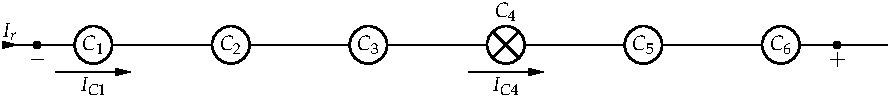
\includegraphics[scale=0.7]{../figs/AsociacionSerieCelulas}
\end{centering}

\caption{Agrupación serie de células con una célula diferente al resto.\label{fig:CelulaSombreada}}

\end{figure}

Cuando esta agrupación serie sea acoplada a una carga quedará polarizada
en un rango de tensiones, lo que ocasionará que cada célula trabaje
en unas condiciones determinadas. En la figura \ref{fig:TensionesCelulaSombreada}
se recoge la relación entre las tensiones que alcanzan las células
1 y 4 para diferentes tensiones de la agrupación. Es evidente que,
mientras la célula 1 está polarizada correctamente, la célula 4 está
sometida a tensiones negativas en la mayor parte del intervalo. 

Esta situación queda aún más patente en la figura \ref{fig:PotenciaCelulasSombreada}.
Mientras la célula 1 trabaja en el cuadrante 1 (entregando potencia),
la célula 4 se convierte en una carga, disipando la potencia del resto
de células. 

Al presentar la ecuación \ref{eq:BalancePotenciasModulo} indicábamos
que la potencia eléctrica adquiría signo positivo y, por tanto, disminuía
el valor de la potencia calorífica a disipar. Sin embargo, en este
caso la potencia eléctrica es negativa lo que implica un incremento
en el calor a disipar. La consecuencia inmediata de este modo de funcionamiento
es la elevación de su temperatura respecto al conjunto de células
del módulo, pudiendo dañar gravemente los materiales encapsulantes
que la rodean. Por este motivo, esta avería es conocida como {}``punto
caliente'' (\emph{hot spot}).


\begin{figure}
\begin{centering}
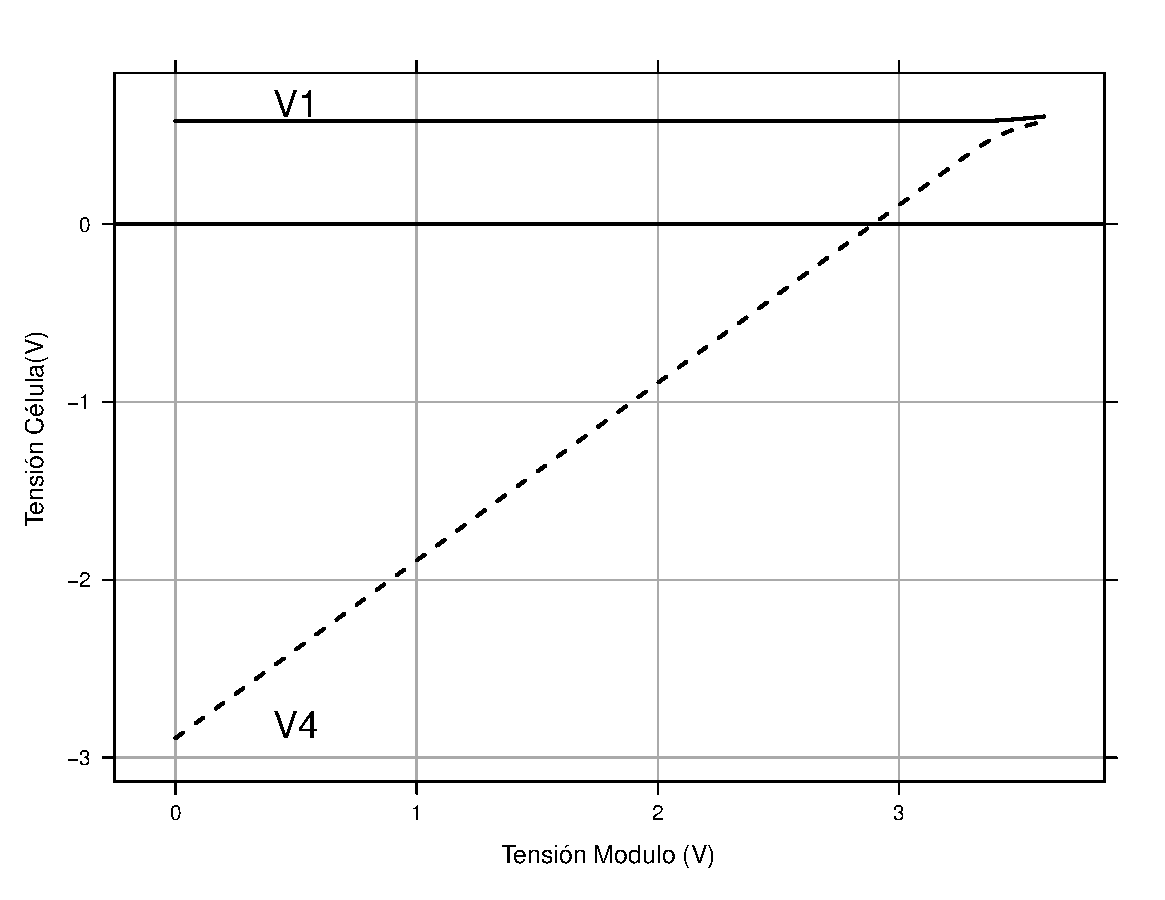
\includegraphics[scale=0.5]{../figs/TensionCelula_Sombras}
\end{centering}

\caption{Tensión de las células 1 y 4 para diferentes tensiones del módulo
definido por la agrupación serie de la figura \ref{fig:CelulaSombreada}.\label{fig:TensionesCelulaSombreada}}

\end{figure}


\begin{figure}
\begin{centering}
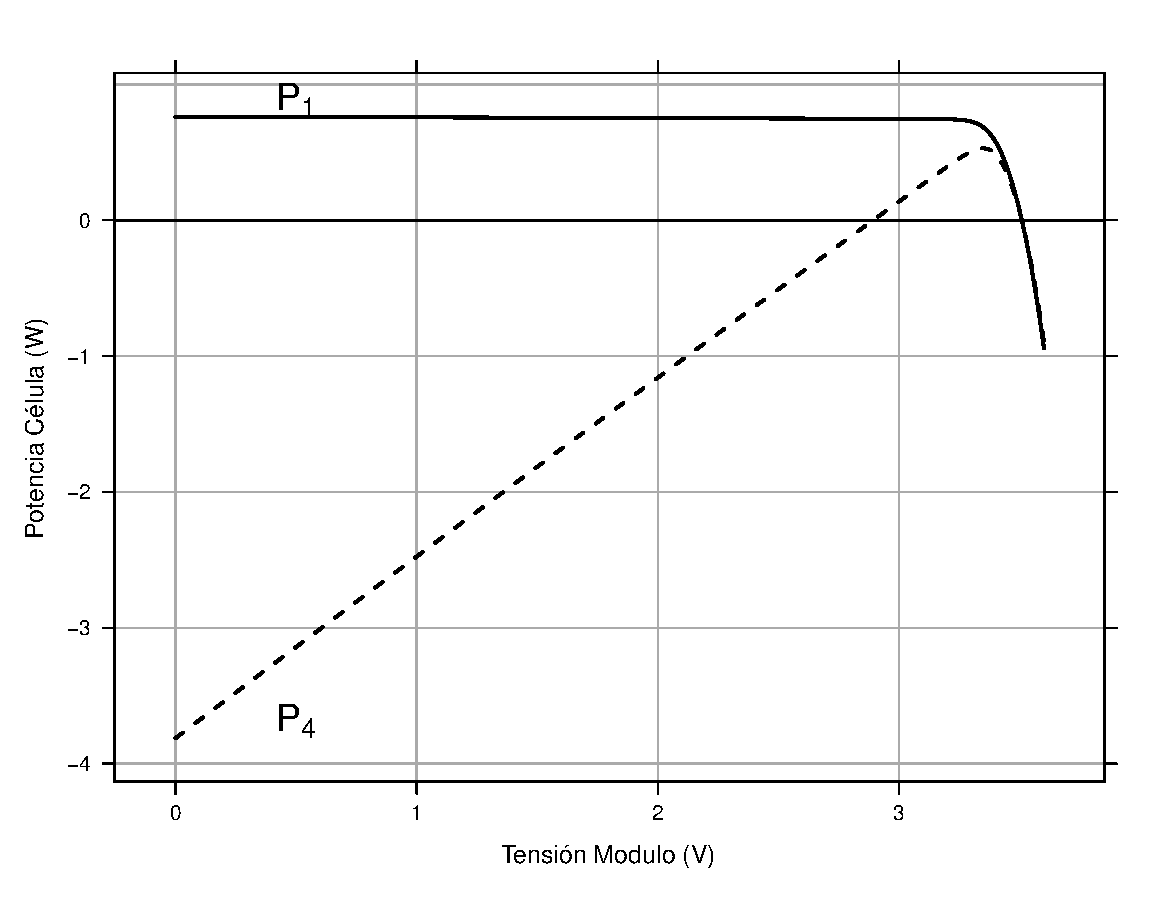
\includegraphics[scale=0.5]{../figs/PotenciaCelula_Sombra}
\end{centering}

\caption{Potencia de las células 1 y 4 para diferentes tensiones del módulo
definido por la agrupación serie de la figura \ref{fig:CelulaSombreada}.\label{fig:PotenciaCelulasSombreada}}

\end{figure}


\subsubsection{Diodo de paso}

Para proteger a la célula sombreada es necesario habilitar un camino
alternativo de corriente y así evitar que trabaje como un receptor
de la potencia del resto de la agrupación. Un método frecuentemente
empleado consiste en incluir diodos de paso conectados en paralelo
con la agrupación serie (figura \ref{fig:DiodosPaso}). 


\begin{figure}
\begin{centering}
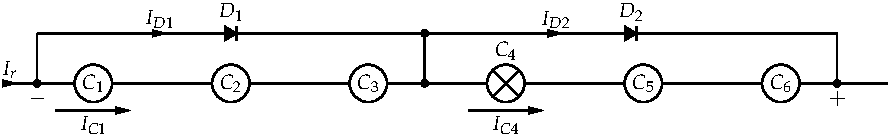
\includegraphics[scale=0.75]{../figs/AsociacionSerieCelulas_DiodosPaso}
\end{centering}

\caption{Colocación de diodo de paso para evitar el fenómeno de punto caliente.\label{fig:DiodosPaso}}

\end{figure}



Con la inclusión de los diodos de paso, la curva corriente-tensión
de la agrupación difiere sensiblemente de la ideal cuando aquellos
se activan. En la figura \ref{fig:CurvaIVDiodosPaso} se representa
las diferentes corrientes que circulan por la agrupación cuando el
funcionamiento de la célula $C_{4}$ obliga al diodo $D_{2}$ a activarse.
Como referencia, en esta figura se incluye la corriente $I_{11}$
, representando la corriente que circularía por la célula $C_{1}$
si la célula $C_{4}$ no presentase problemas. Durante un rango de
tensiones el diodo $D_{2}$permanece activado, conduciendo la corriente
que la célula $C_{4}$ no puede. A partir de un punto determinado,
el diodo queda polarizado en inversa y deja de conducir, limitando
la corriente que puede circular por la serie.


\begin{figure}
\begin{centering}
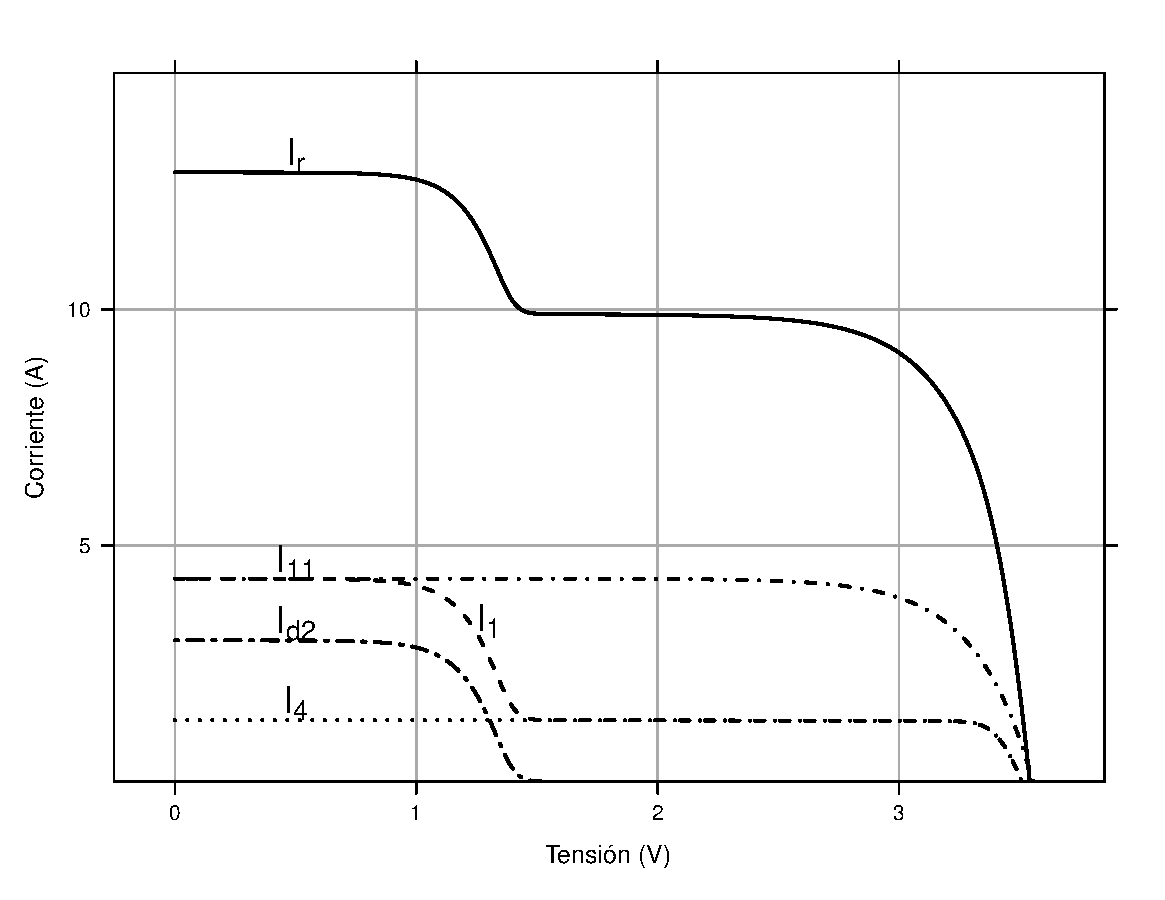
\includegraphics[scale=0.5]{../figs/CurvaIV_DiodoPaso}
\end{centering}

\caption{Curva corriente-tensión de la agrupación serie de la figura \ref{fig:DiodosPaso}.
La corriente $I_{11}$ representa la corriente que circularía por
la célula $C_{1}$ si la célula $C_{4}$ no presentase problemas.\label{fig:CurvaIVDiodosPaso}}

\end{figure}

Gracias al diodo de paso, la tensión que debe soportar ahora la célula
$C_{4}$ es sustancialmente inferior a la obtenida sin diodos, tal
y como se observa en la figura \ref{fig:TensionesDiodosPaso}. Si
se compara esta figura con la figura \ref{fig:TensionesCelulaSombreada},
se comprueba que la activación del diodo $D_{2}$ limita la tensión
negativa en la célula $C_{4}$. A partir de un punto, la protección
ya no es necesaria y este diodo se desactiva con lo que la tensión
de la célula $C_{4}$ queda nuevamente a merced del conjunto. 


\begin{figure}
\begin{centering}
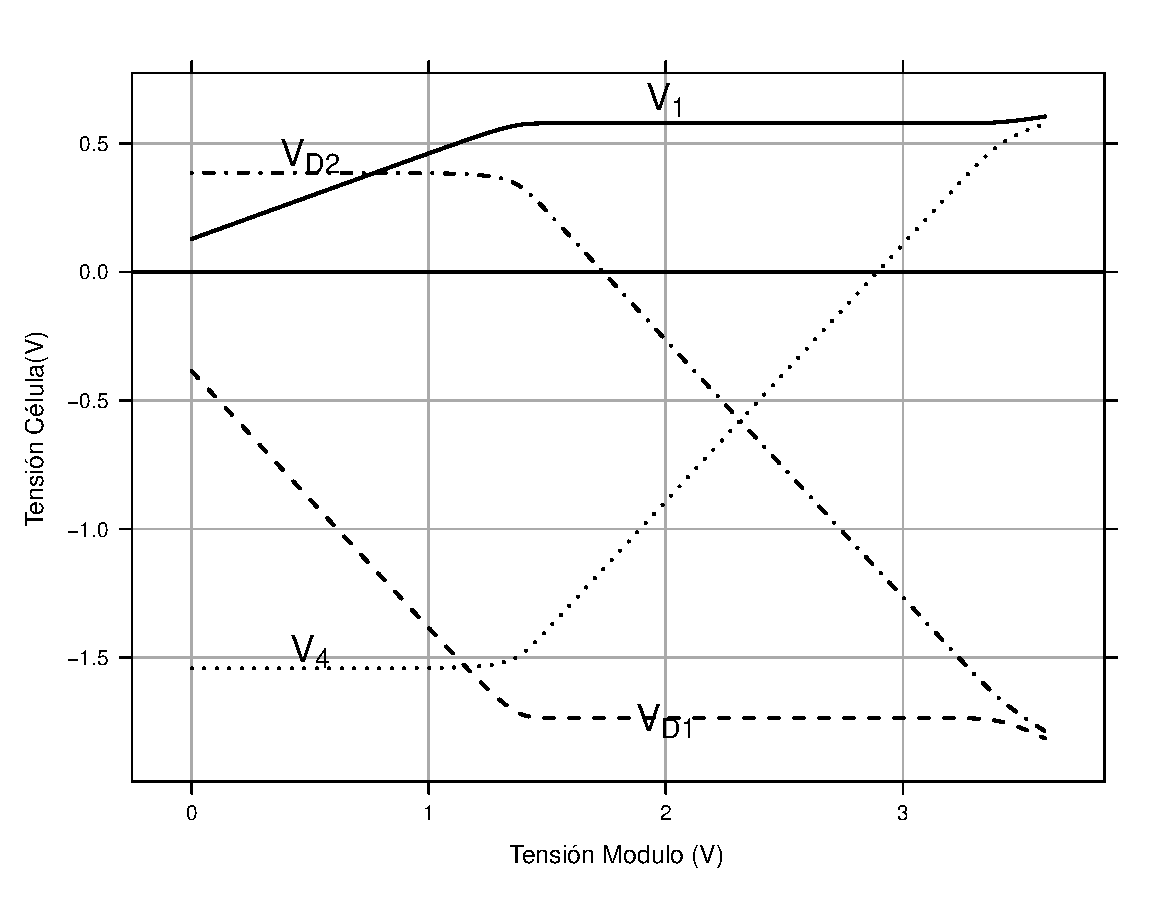
\includegraphics[scale=0.5]{../figs/TensionesCelulasDiodos_DiodoPaso}
\end{centering}

\caption{Tensiones en los elementos de la figura \ref{fig:DiodosPaso} para
diferentes tensiones de la agrupación serie.\label{fig:TensionesDiodosPaso}}

\end{figure}

Sin embargo, como se recoge en la figura \ref{fig:PotenciaDiodosPaso},
también se reduce la potencia en la célula $C_{4}$ gracias a la actuación
del diodo $D_{2}$, que debe asumir esta potencia desviada durante
su activación. Dado que las células protegidas por el diodo $D_{1}$
funcionan sin problemas aparentes, este diodo permanece polarizado
en inversa durante todo el intervalo. Sin embargo, el funcionamiento
combinado de la célula $C_{4}$ y su diodo asociado alteran la curva
de potencia-tensión del resto de células (véase la correspondiente
a $C_{1}$ en la figura \ref{fig:PotenciaDiodosPaso}) y de la agrupación,
como es evidente en la figura \ref{fig:PotenciaTensionSerieDiodosPaso}. 

Si representamos el número de células asociadas a un diodo de paso
con $N_{D}$\nomenclature[Nd]{$N_{D}$}{Número de células asociadas a un diodo de paso}\nomenclature[Gs]{$G_{s}$}{Radiación recibida por una célula sombreada},
y la radiación que recibe la célula diferente con $G_{s}$, es posible
calcular la diferencia de temperatura entre la célula afectada y el
resto. El balance de potencias de la ecuación \ref{eq:BalancePotenciasModulo}
aplicado a la célula diferente es:

\begin{equation}
A_{c}\cdot G_{s}=-(N_{D}-1)\eta\cdot A_{c}\cdot G_{ef}+P_{Qs}\label{eq:BalancePotenciasCelulaDiferente}\end{equation}
y aplicado a las células que funcionan correctamente es:\begin{equation}
A_{c}\cdot G_{ef}=\eta\cdot A_{c}\cdot G_{ef}+P_{Q}\label{eq:BalancePotenciasCelulasCorrectas}\end{equation}
donde $\eta$ representa la eficiencia de las células que funcionan
correctamente. La diferencia de temperaturas entre la célula diferente
y el resto de células viene dado por la ecuación  \ref{eq:TcPotenciaCalorifica}:\begin{equation}
T_{cs}-T_{c}=\frac{C_{T}}{A_{c}}\cdot(P_{Qs}-P_{Q})\label{eq:DiferenciaTemperaturas}\end{equation}
\nomenclature[Tcs]{$T_{cs}$}{Temperatura de funcionamiento de una célula sombreada}

Sustituyendo las ecuaciones \ref{eq:BalancePotenciasCelulaDiferente}
y \ref{eq:BalancePotenciasCelulasCorrectas}, y operando adecuadamente
se obtiene:\begin{equation}
T_{cs}-T_{c}=C_{T}\cdot\left[\left(G_{s}-G_{ef}\right)+N_{D}\cdot\eta\cdot G_{ef}\right]\end{equation}
cuyo valor máximo ocurre cuando la radiación que recibe la célula
diferente es igual al resto, $G_{s}=G_{ef}$:

\begin{equation}
T_{cs}-T_{c}=C_{T}\cdot N_{D}\cdot\eta\cdot G_{ef}\label{eq:DiferenciaTemperaturasArreglada}\end{equation}


Para un módulo convencional, $N_{D}=18$, $C_{T}=\SI{0.036}{\celsius\per\watt\per\meter\squared}$\nomenclature[Ct]{$C_{T}$}{Coeficiente térmico de un módulo}
y $\eta=0.14$, la diferencia de temperaturas entre dos células protegidas
por un diodo es $T_{cs}-T_{c}=0.091\cdot G_{ef}$ . Para una radiación
$G_{ef}=\SI{1000}{\watt\per\meter\squared}$se obtiene un valor aproximado
de $\SI{91}{\celsius}$. Si el módulo no incluyese diodos de paso,
la diferencia de temperaturas vendría dada por:\begin{equation}
T_{cs}-T_{c}=C_{T}\cdot N_{cs}\cdot\eta\cdot G_{ef}\label{eq:DiferenciaTemperaturasSinDiodo}\end{equation}
siendo $N_{cs}$ el número de células en serie. Para un módulo de
36 células en serie, la misma radiación del caso anterior provocaría
una diferencia de temperaturas superior a los $\SI{180}{\celsius}$.


\begin{figure}
\begin{centering}
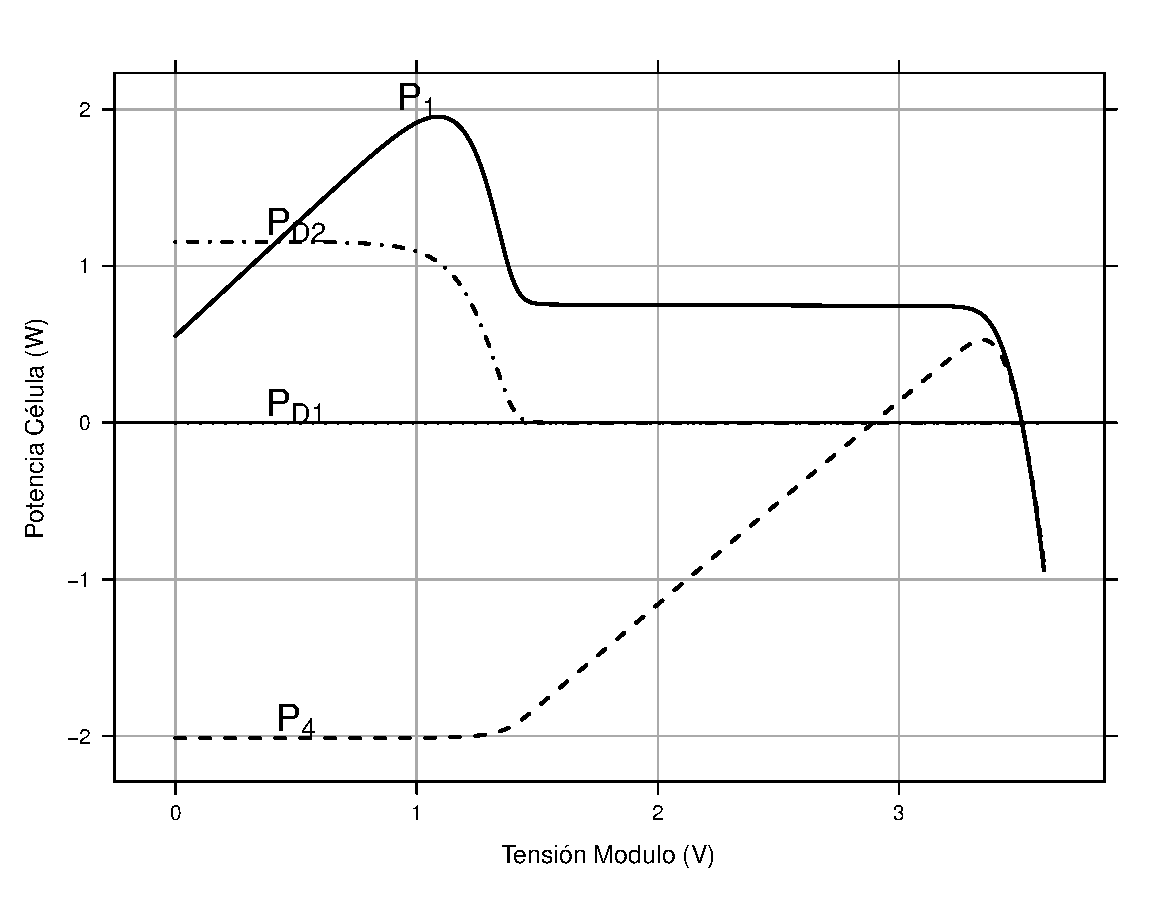
\includegraphics[scale=0.5]{../figs/PotenciaCelulas_DiodoPaso}
\end{centering}

\caption{Potencias de los elementos de la figura \ref{fig:DiodosPaso} para
diferentes tensiones de la agrupación serie.\label{fig:PotenciaDiodosPaso}}

\end{figure}


Por otra parte, la alteración de esta curva produce dos máximos de
potencia, uno local y otro absoluto. Ante estos dos puntos un algoritmo
de búsqueda del punto de máxima potencia, como los descritos en el
apartado \ref{sub:BusquedaMPP}, puede ofrecer respuestas erróneas.


\begin{figure}
\begin{centering}
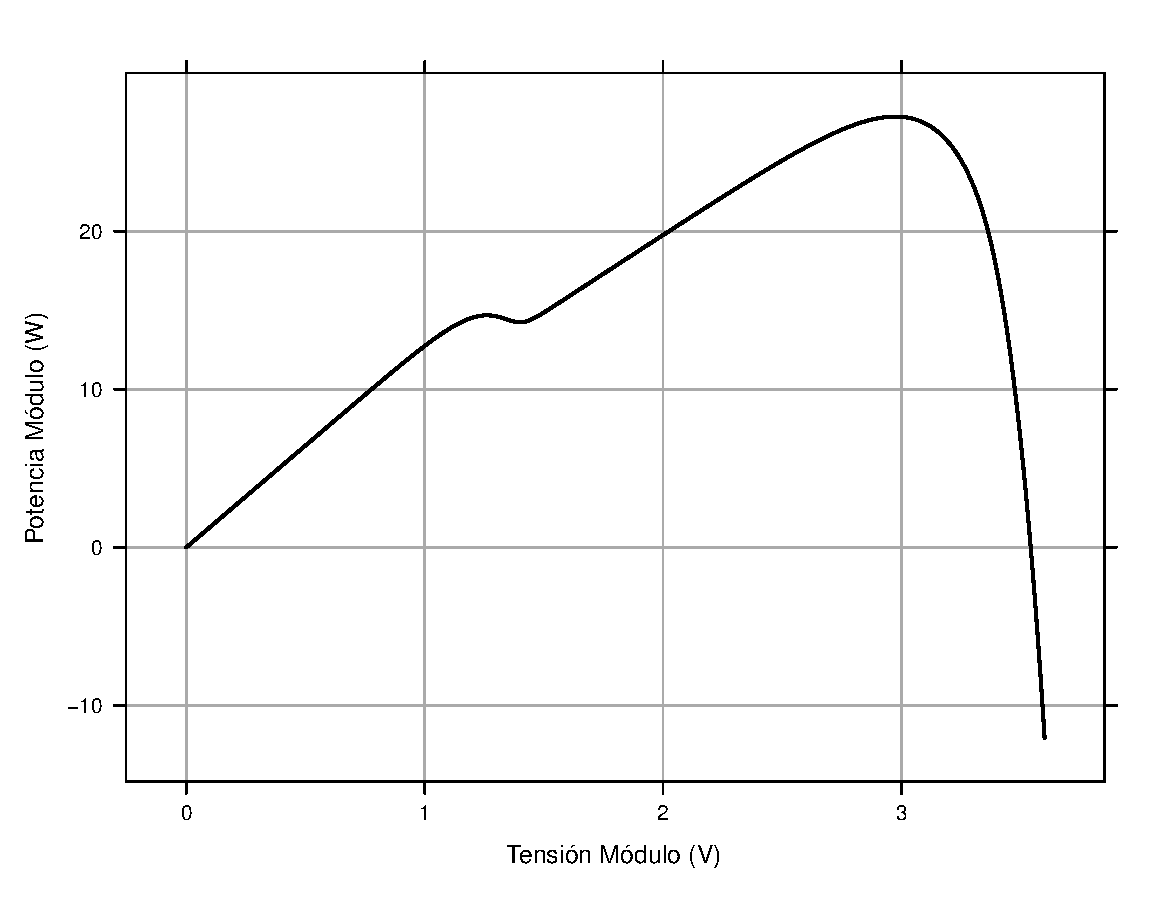
\includegraphics[scale=0.5]{../figs/PotenciaModulo}
\end{centering}

\caption{Curva potencia-tensión de la agrupación serie de la figura figura
\ref{fig:DiodosPaso} cuando la célula $C_{4}$ presenta problemas
de funcionamiento.\label{fig:PotenciaTensionSerieDiodosPaso} }

\end{figure}

En los módulos comerciales suele optarse por proteger de 18 a 20 células
con un diodo de paso. Se suele preferir conexiones solapadas como
la mostrada en la figura \ref{fig:ConexionTipicaDiodosPaso} para
evitar el cortocircuito del módulo cuando los dos diodos conducen
simultáneamente y ante un cambio de polaridad en la conexión del módulo.


\begin{figure}
\begin{centering}
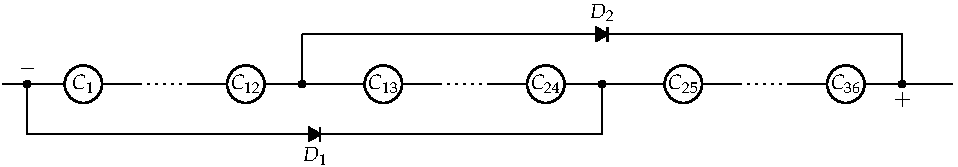
\includegraphics{../figs/AsociacionSerieCelulas_DiodosPasoAlternos}
\end{centering}

\caption{Configuración típica de conexión de diodos de paso en una serie de
36 células.\label{fig:ConexionTipicaDiodosPaso}}

\end{figure}

El análisis del {}``punto caliente'' recogido en la literatura ha
estado ligado comúnmente a células averiadas o afectadas por sombra.
En tiempos recientes se ha puesto de manifiesto la problemática asociada
a ciertos niveles de dispersión de parámetros de células en un mismo
módulo. En determinadas condiciones, el funcionamiento de este tipo
de módulos también provoca la aparición de puntos calientes con gradientes
elevados de temperatura, recortando así su vida útil \cite{Lorenzo.Martinez.ea2009}.


\section{Generador Fotovoltaico}

Un generador fotovoltaico es una asociación eléctrica de módulos fotovoltaicos
para adaptarse a las condiciones de funcionamiento de una aplicación
determinada. Se compone de un total de $N_{p}\cdot N_{s}$ módulos,
siendo $N_{p}$ el número de ramas y $N_{s}$ el número de módulos
en cada serie. El número de ramas define la corriente total del generador,
$I_{g}=N_{p}\cdot I_{m}$, y el número de módulos por serie define
la tensión del generador, $V_{g}=N_{s}\cdot V_{m}$\nomenclature[Vg]{$V_{g}$}{Tensión de un generador}\nomenclature[Ig]{$I_{g}$}{Corriente de un generador}
. La figura \ref{fig:EsquemaGenerador} muestra un generador fotovoltaico
compuesto por 2 ramas de 3 módulos en serie. Sin embargo, al considerar
las características reales de los módulos que componen un generador
fotovoltaico es necesario analizar un fenómeno que altera estos cálculos
sencillos: las pérdidas por dispersión de parámetros.


\begin{figure}
\begin{centering}
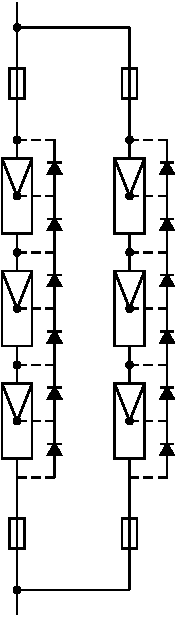
\includegraphics[angle=270]{../figs/AsociacionModulos}
\end{centering}

\caption{Esquema de un generador fotovoltaico compuesto por 2 ramas de 3 módulos
en serie. El esquema incluye la protección con fusibles y por rama
y los diodos de paso incluidos en cada módulo.\label{fig:EsquemaGenerador}}

\end{figure}


\subsection{Pérdidas por dispersión}

Los parámetros eléctricos de los módulos fotovoltaicos que componen
un generador nunca son exactamente iguales. La dispersión de estos
parámetros provoca que la potencia eléctrica total sea inferior a
la suma de las individuales.

Para abordar el cálculo del comportamiento del generador es preciso
emplear herramientas de análisis estadístico. Según \cite{Zilles1993}
la corriente de máxima potencia de un conjunto de módulos puede caracterizarse
por una distribución tipo Weibull:\begin{equation}
f(I_{mpp})=\alpha\beta^{-\alpha}I_{mpp}^{\alpha-1}exp\left[-\left(\frac{I_{mpp}}{\beta}\right)^{\alpha}\right]\end{equation}
siendo $\alpha$ el factor de forma y $\beta$ el factor de escala
de la distribución. La eficiencia de conexión serie es:\begin{equation}
\eta_{cs}=\frac{I_{mpp}^{r}}{\overline{I_{mpp}}}\end{equation}
\nomenclature[etacs]{$\eta_{cs}$}{Eficiencia de la conexión serie en un generador}donde
$I_{mpp}^{r}$ es la corriente de la rama, y $\overline{I_{mpp}}$
la media de las corrientes del grupo de módulos. A partir de la distribución
y la definición de eficiencia de conexión serie puede deducirse que
ésta se calcula mediante\begin{equation}
\eta_{cs}=N_{s}^{-\frac{1}{\alpha}}\label{eq:EficienciaConexionSerie}\end{equation}
siendo $N_{s}$ el número de módulos en la serie. Por otra parte,
puede demostrarse que la tensión de un grupo de módulos puede modelarse
mediante una función gaussiana y que la dispersión de valores de tensión
es suficientemente baja para poder considerar que la eficiencia de
conexión de ramas en paralelo es igual a 1. 

Según la ecuación \ref{eq:EficienciaConexionSerie} la eficiencia
de la conexión serie disminuye si aumenta $N_{s}$. Así, para reducir
las pérdidas por dispersión es aconsejable el uso de series cortas.
Sin embargo, esta opción implica trabajar con tensiones bajas que
pueden conducir a grandes secciones de cableado en sistemas de gran
potencia. 

Asimismo, la eficiencia aumenta con $\alpha$. La dispersión de valores
de un conjunto modelado por una distribución tipo Weibull depende
inversamente del valor de $\alpha$. Por tanto, un método para reducir
las pérdidas por dispersión consiste en realizar clasificaciones de
los módulos atendiendo a sus valores reales de corriente. En sistemas
de cierta entidad, puede ser conveniente realizar una clasificación
en dos o tres categorías y componer cada rama con módulos pertenecientes
a una misma categoría. Este método puede, teóricamente, conllevar
reducciones del 2-3\% en las pérdidas globales del sistema. 

La base de partida para realizar las clasificaciones es la información
suministrada por el fabricante de los módulos. Esta información (habitualmente
conocida como {}``flash-list'') consiste en un conjunto de medidas
eléctricas para cada uno de los módulos. Estas medidas se realizan
en una cámara oscura en la que se sitúa el módulo para iluminarlo
durante un breve lapso de tiempo (de ahí el nombre de {}``flash'')
simulando su funcionamiento a sol real. La indeterminación asociada
a este método en relación a las medidas a sol real son del mismo rango
que la separación entre categorías. Como ha sido puesto de relieve
recientemente en el contexto de controles de calidad de plantas fotovoltaicas
\cite{Lorenzo.Moreton.ea2008}, estas medidas conllevan un error
asociado que limitan su aplicación para la construcción de las categorías
de módulos. En esta experiencia se demostró que la desviación estándar
de las diferencias entre los valores recogidos en el {}``flash-list''
y los obtenidos a sol real era similar a la anchura de las categorías
necesarias para clasificar los módulos. Por tanto, aunque la clasificación
es aconsejable desde el punto de vista teórico, su práctica queda
cuestionada seriamente cuando emplea como material de partida las
medidas tipo {}``flash''.

%%% Local Variables:
%%% mode: LaTex
%%% TeX-master: "ESF.tex"
%%% End: 